% Author: Dominik Harmim <harmim6@gmail.com>

\documentclass[a4paper, 11pt]{article}

\usepackage[british]{babel}
\usepackage[utf8]{inputenc}
\usepackage[T1]{fontenc}
\usepackage[left=2cm, top=3cm, text={17cm, 24cm}]{geometry}
\usepackage{graphicx}
\usepackage[unicode, colorlinks, hypertexnames=false, citecolor=red]{hyperref}
\usepackage{amsmath, amsthm, amssymb}
\usepackage{mathtools}
\usepackage[inline]{enumitem}
\usepackage{dirtytalk}
\usepackage{listings}
\usepackage{xcolor}
\usepackage{multirow}


\hypersetup{
    pdftitle={Static Analysis and Verification - Project - PRISM},
    pdfauthor={Dominik Harmim <xharmi00@stud.fit.vutbr.cz>}
}

\graphicspath{{img/}}

\setlength{\parindent}{0pt}
\setlength{\parskip}{.5 \bigskipamount}

\theoremstyle{definition}
\newtheorem{definition}{Definition}[section]

\definecolor{bluekeywords}{rgb}{.13, .13, 1}
\definecolor{greencomments}{rgb}{0, .5, 0}
\lstset{
    basicstyle=\ttfamily,
    backgroundcolor=\color{white},
    columns=fullflexible,
    captionpos=b,
    tabsize=4,
    keepspaces=true,
    numbers=left,
    xleftmargin=1.5em,
    frame=single
}
\lstdefinelanguage{prism}{
    showspaces=false,
    showtabs=false,
    breaklines=true,
    showstringspaces=false,
    breakatwhitespace=true,
    commentstyle=\color{greencomments},
    keywordstyle=\color{bluekeywords},
    comment=[l] {//},
    morecomment=[s]{/*}{*/},
    keywords={%
        bool, int, double, ctmc, dtmc, mdp, pta, module, endmodule,
        rewards, endrewards, const, true, false, formula, label,
        init, system, endsystem, invariant, endinvariant, global,
        endinit, min, max, floor, ceil, round, pow, mod, log%
    }
}


\begin{document}


\begin{titlepage}
    \begin{center}
        \textsc{%
            \LARGE{Brno University of Technology} \\
            \smallskip
            \Large{Faculty of Information Technology}%
        }

        \includegraphics[width=.77 \linewidth]{FIT-logo.pdf}

        \vspace{\stretch{.382}}

        \Huge{Static Analysis and Verification} \\
        \LARGE{\textbf{Project\,---\,PRISM}} \\[1.5em]
        \includegraphics[width=.1 \linewidth]{prism-logo.png}

        \vspace{\stretch{.618}}
    \end{center}

    {\Large%
        \today
        \hfill
        Dominik Harmim (\texttt{xharmi00})%
    }
\end{titlepage}


\clearpage
\pagenumbering{roman}
\setcounter{page}{1}
\tableofcontents


\clearpage
\pagenumbering{arabic}
\setcounter{page}{1}


\section{Introduction}

This project aims to study a~selected software tool for \emph{static
analysis and verification}, do some experiments with the tool, and
describe it appropriately. It was selected
\textbf{PRISM}\,---\,a~\emph{probabilistic model checker.}

The rest of the essay is organised as follows. Chapter~\ref{sec:prism}
describes PRISM and its principles. Chapter~\ref{sec:caseStud} then
deals with a~reproduction of publicly available case studies. In
Chapter~\ref{sec:customExp}, there are discussed made custom experiments.
Finally, Chapter~\ref{sec:con} concludes the essay.


\section{\texorpdfstring{PRISM\,---\,Probabilistic Model Checker}{%
    PRISM - Probabilistic Model Checker%
}}
\label{sec:prism}

This Chapter describes PRISM\,---\,a~\emph{probabilistic model
checker}\,---\,and its principles, usage, used algorithms, \emph{modelling
language}, implementation, theory it is based on, etc. The description
of \emph{model checking} in general together with the definition of
fundamentals of \emph{temporal logic} and basic concepts in model checking
can be found in books~\cite{principlesOfModelCheck, handbookOfModelCheck}.
This Chapter is based on papers~\cite{stochModelCheck,
advancesOfProbabModelCheck} where are discussed principles and algorithms
that is PRISM based on, implementation of these algorithms in PRISM, and
related theory. Some of the mentioned algorithms are in more detail covered
in~\cite{automatedVerForProbSys}. The most recent features of PRISM
(mainly \emph{probabilistic timed automata}) are introduced in the PRISM
tool paper~\cite{prism40}. Some information was also acquired from
a~web page of PRISM\footnote{\label{fn:prism}A~web page of
a~\emph{probabilistic model checker} \textbf{PRISM}:
\url{http://www.prismmodelchecker.org}.}. Further details about
\emph{probabilistic systems} and perhaps more formal and theoretic insight
is available at Chapter~10 of~\cite{principlesOfModelCheck} and
Chapter~28 of~\cite{handbookOfModelCheck}. Moreover, it was used information
and other materials from lecture slides~\cite{bissLec, esslliLec,
probModelCheckLec, mbaCeska}.

PRISM\textsuperscript{\ref{fn:prism}} is a~\emph{probabilistic model checker}
developed mainly at the University of Birmingham by David Parker, the
University of Glasgow by Gethin Norman, and the University of Oxford by
Marta Kwiatkowska. It is \emph{free} and \emph{open-source} (released under
the GNU General Public License). It is available for Linux, Unix, macOS, and
Windows. It accepts \emph{probabilistic models} described in its
\emph{modelling language}\,---\,a~simple, high-level state-based language
further described in Chapter~\ref{sec:prisimLang}. Three types of
probabilistic models (see Chapter~\ref{sec:probModels}) are supported
directly; these are \emph{discrete-time Markov chains (DTMCs)},
\emph{continuous-time Markov chains (CTMCs)}, and \emph{Markov decision
processes (MDPs)}, i.e., \emph{probabilistic automata (PAs)}. Additionally,
\emph{probabilistic timed automata (PTAs)} are partially supported, with the
subset of diagonal-free PTAs supported directly via \emph{digital clocks}.
Note that since version 4.0 of PRISM~\cite{prism40}, PTAs are fully
supported. Also, \emph{priced} PTAs are supported, i.e., PTAs augmented
with \emph{costs} and \emph{rewards}. PTAs are finite-state automata
enriched with real-valued clocks, in the style of \emph{timed automata}
(defined in~\cite{principlesOfModelCheck}), and with discrete probabilistic
choice, in the style of MDPs. So, PTAs can be viewed as DTMCs with
\emph{continuous-time} and \emph{non-determinism}.

Properties are formally specified using \emph{probabilistic computation
tree logic (PCTL)} for DTMCs and MDPs, and \emph{continuous stochastic
logic (CSL)} for CTMCs. These are discussed in Chapter~\ref{sec:prismLogics}.
PTAs have \emph{probabilistic timed computation tree logic (PTCTL)}, an
extension of \emph{timed computation tree logic (TCTL)} defined
in~\cite{principlesOfModelCheck}.

PRISM first parses the model description and constructs an internal
representation of the probabilistic model, computing the \emph{reachable
state-space} of the model and discarding any unreachable states. The resulting
model represents the set of all \emph{feasible configurations} which can arise
in the modelled system. This process is depicted in
Figure~\ref{fig:prismModelConstruction}. Next, the specification is parsed, and
appropriate model checking algorithms are performed on the model by induction
over syntax. The whole process is outlined in
Figure~\ref{fig:prismOverview}. In some cases, such as for properties
which include a~\emph{probability bound}, PRISM will report
a~\texttt{True/False} outcome, indicating whether or not each property is
satisfied by the current model. More often, however, properties return
\emph{quantitative} results and PRISM reports, e.g., the actual probability
of a~specific event occurring in the model. Furthermore, PRISM supports the
notion of \emph{experiments}, which is a~way of automating multiple instances
of model checking. These allow one to quickly obtain the outcome of one or
more properties as functions of model and property parameters. The resulting
table of values can either be viewed directly, exported for use in an
external application, or plotted as a~graph. Moreover, PRISM incorporates
substantial graph-plotting functionality. It is often a~handy way
of identifying interesting patterns or trends in the behaviour of a~system.

\begin{figure}[hbt]
    \centering

    \begin{minipage}{.49 \linewidth}
        \centering
        \includegraphics[width=.9 \linewidth]{prism-overview.png}
        \caption{%
            Overview of the workflow of PRISM~\cite{probModelCheckLec}%
        }
        \label{fig:prismOverview}
    \end{minipage}
%
    \begin{minipage}{.49 \linewidth}
        \centering
        \includegraphics[width=.9 \linewidth]{prism-model-construction.png}
        \caption{%
            Overview of the model construction process in
            PRISM~\cite{probModelCheckLec}%
        }
        \label{fig:prismModelConstruction}
    \end{minipage}
\end{figure}

Figure~\ref{fig:prismGui} shows a~screenshot of the PRISM graphical user
interface, illustrating the results of a~model checking experiment being
plotted on a~graph. The tool also features a~built-in text-editor for the
PRISM language and a~\emph{simulator} for model debugging. Alternatively, all
model checking functionality is also available in a~command-line version of
the tool.

\begin{figure}[hbt]
    \centering
    \includegraphics[width=.7 \linewidth]{prism-gui.png}
    \caption{%
        A~screenshot of the PRISM graphical user interface \\
        (\url{http://www.prismmodelchecker.org/screenshots.php})%
    }
    \label{fig:prismGui}
\end{figure}

\subsection{Probabilistic Models}
\label{sec:probModels}

This Chapter briefly describes and formally defines three major types of
\emph{probabilistic models} supported by PRISM. For particular algorithms
that reason about the  probability of certain events occurring in such models
see~\cite{automatedVerForProbSys, stochModelCheck}. In more detail, the
models are covered in~\cite{principlesOfModelCheck, handbookOfModelCheck,
automatedVerForProbSys, stochModelCheck}.

\subsubsection{Discrete-Time Markov Chains (DTMCs)}

\textbf{Discrete-time Markov chains (DTMCs)} model systems whose behaviour
at each point in time can be described by a~\emph{discrete probabilistic
choice} over several possible outcomes. Essentially, a~DTMC can be thought
of as a~\emph{labelled state-transition system} in which each transition is
annotated with a~probability value indicating a~likelihood of its occurrence.
That is to say, the successor state of state~$ s $, say, is chosen according
to a~\emph{probability distribution}. This probability distribution only
depends on the current state~$ s $, and not, e.g., the path fragment that
led to state~$ s $ from some initial state. Accordingly, the system
evolution does not depend on the history (i.e., the path fragment that
has been executed so far), but only on the current state~$ s $. This is
known as the \emph{memory-less property}. Intuitively, DTMC is defined by
\begin{enumerate*}[label={(\roman*)}]
    \item
        states\,---\,\emph{set of states} representing possible
        configurations of the system being modelled,

    \item
        transitions\,---\,transitions between states model evolution of
        system's state; occur in \emph{discrete time-steps},

    \item
        and probabilities\,---\,probabilities of making transitions
        between states are given by discrete probability distributions.
\end{enumerate*}

\begin{definition}[DTMC]
Formally, a~(labelled) DTMC~$ \mathcal{D} $ is a~tuple $ (S, s_{init},
\boldsymbol{P}, AP, L) $ where:
\begin{itemize}
    \item
        $ S $~is a~(countable non-empty) set of \emph{states}
        (\emph{state-space});

    \item
        $ s_{init} \in S $ is the \emph{initial state} (can be
        generalised to an \emph{initial distribution} $ \iota_{init} : S
        \rightarrow [0, 1] $, such that $ \sum_{s \in S} \iota_{init}(s)
        = 1 $);

    \item
        $ \boldsymbol{P} : S \times S \rightarrow [0, 1] $ is the
        \emph{transition probability matrix} such that $ \sum_{s^\prime
        \in S} \boldsymbol{P}(s, s^\prime) = 1 $ for all $ s \in S $;

    \item
        $ AP $ is a~set of \emph{atomic prepositions};

    \item
        $ L : S \rightarrow 2^{AP} $ is a~\emph{labelling function} that
        assigns, to each state $ s \in S $, a~set $ L(s) $ of
        \emph{atomic prepositions}.
\end{itemize}
\end{definition}

For a~state $ s \in S $ of a~DTMC~$ \mathcal{D} $, the probability of
moving to a~state $ s^\prime \in S $ in one discrete step is given
by $ \boldsymbol{P}(s, s^\prime) $. An (infinite) \emph{path}
of~$ \mathcal{D} $, which gives one possible evolution of the Markov chain,
is a~non-empty alternating (infinite) sequence of states $ s_0 s_1 s_2
\ldots \in S^\omega $ such that $ \boldsymbol{P}(s_i, s_{i + 1}) > 0 $ for
all $ i \geq 0 $.

Alternatively, a~DTMC can be defined as a~\emph{family of random variables}
$ \{X(k)\ |\ k = 0, 1, 2, \ldots\} $ where $ X(k) $ are observations at
discrete time-steps, i.e., $ X(k) $ is the state of the system at
time-step~$ k $. This satisfies the \emph{Markov property} (memory-less
property): $ Pr(X(k) = s_k\ |\ X(k - 1) = s_{k - 1}, \ldots, X(0) = s_0)
= Pr(X(k) = s_k\ |\ X(k - 1) = s_{k - 1}) $, i.e., for a~given current
state, future states are independent of past.

\subsubsection{Continuous-Time Markov Chains (CTMCs)}

DTMCs are \emph{discrete-time} models: the progress of time is modelled
by discrete time steps, one for each transition of the model. For many
systems, it is preferable to use a~\emph{continuous} model of time, where
the delays between transitions can be arbitrary real values. One popular
model is a~\textbf{continuous-time Markov chain (CTMC)}, in which
transition delays are assumed to be modelled by \emph{exponential
distributions}.

\begin{definition}[CTMC]
Formally, a~(labelled) CTMC~$ \mathcal{C} $ is a~tuple $ (S, s_{init},
\boldsymbol{R}, AP, L) $ where:
\begin{itemize}
    \item
        $ S $, $ s_{init} \in S $, $ AP $, and $ L : S \rightarrow
        2^{AP} $ are as for DTMCs;

    \item
        $ \boldsymbol{R} : S \times S \rightarrow \mathbb{R}_{\geq 0} $
        is the \emph{transition rate matrix}.
\end{itemize}
\end{definition}

The matrix~$ \boldsymbol{R} $ assigns a~\emph{rate} to each pair of
states in the CTMC. A~transition can only occur between states~$ s $
and~$ s^\prime $ if $ \boldsymbol{R}(s, s^\prime) > 0 $ and, in this
case, the delay before the transition can occur is modelled as an
exponential distribution with rate $ \boldsymbol{R}(s, s^\prime) $,
i.e., the probability of this transition being triggered within~$ t $
time-units is $ 1 - e^{-\boldsymbol{R}(s, s^\prime) \cdot t} $.
Usually, in a~state~$ s $, there is more than one state~$ s^\prime $
for which $ \boldsymbol{R}(s, s^\prime) > 0 $, which is referred to
as a~\emph{race condition}. The first transition to be triggered
determines the next state of the CTMC. The time spent in state~$ s $,
before any such transition occurs, is exponentially distributed with
rate $ E(s) $, where: $ E(s) = \sum_{s^\prime \in S} \boldsymbol{R}(s,
s^\prime) $. $ E(s) $ is known as the \emph{exit rate} of state~$ s $.
It can also be determined the actual probability of each
state~$ s^\prime $ being the next state to which a~transition is made
from state~$ s $, independent of the time at which this occurs. This is
defined by the \emph{embedded} DTMC of~$ \mathcal{C} $, which is
$ emb(\mathcal{C}) = (S, s_{init}, \boldsymbol{P}^{emb(\mathcal{C})}, AP,
L) $, where for $ s, s^\prime \in
S $:
$$
    \boldsymbol{P}^{emb(\mathcal{C})}(s, s^\prime) =
    \begin{cases}
        \frac{\boldsymbol{R}(s, s^\prime)}{E(s)}
            & \text{if\ } E(s) \neq 0 \\
        1 & \text{if\ } E(s) = 0 \wedge s = s^\prime \\
        0 & \text{otherwise.}
    \end{cases}
$$
The behaviour of the CTMC can be considered in an alternative way using the
above definitions. It will remain in a~state~$ s $ for a~delay which
is exponentially distributed with rate $ E(s) $ and then make a~transition.
The probability that this transition is to state~$ s^\prime $ is given by
$ \boldsymbol{P}^{emb(\mathcal{C})}(s, s^\prime) $. An (infinite) path
of~$ \mathcal{C} $ is a~non-empty (infinite) sequence $ s_0 t_0 s_1 t_1 s_2
t_2 \ldots \in (S \times \mathbb{R}_{\geq 0})^\omega $ where
$ \boldsymbol{R}(s_i, s_{i + 1}) > 0 $ for all $ i \geq 0 $.
The value~$ t_i $ represents the amount of \emph{time spent} in the
state~$ s_i $.

As for DTMCs, a~CTMC can be alternatively defined as a~family of random
variables $ \{X(t)\ |\ t \in \mathbb{R}_{\geq 0}\} $ where $ X(t) $ are
observations made at time instant~$ t $, i.e., $ X(t) $ is the state of
the system at time instant~$ t $. Furthermore, again, it satisfies the
Markov property.

\subsubsection{Markov Decision Processes (MDPs)}

DTMCs represent a~\emph{fully probabilistic} model of a~system, i.e., in
each state of the model, the exact probability of moving to each other
state is always known. In many instances, this does not realistically model
a~system's behaviour, because it behaves in a~\emph{non-deterministic}
fashion. \textbf{Markov decision processes (MDPs)} (similar to
\emph{probabilistic automata}) are one of the most common formalisms for
modelling systems with both probabilistic and non-deterministic behaviour.

\begin{definition}[MDP]
Formally, a~(labelled) MDP~$ \mathcal{M} $ is a~tuple $ (S, s_{init},
Act, \boldsymbol{P}, AP, L) $ where:
\begin{itemize}
    \item
        $ S $, $ s_{init} \in S $, $ AP $, and $ L : S \rightarrow 2^{AP} $
        are as for DTMCs;

    \item
        $ Act $ is a~(finite non-empty) set of \emph{action labels};

    \item
        $ \boldsymbol{P} : S \times Act \times S \rightarrow [0, 1] $ is
        the \emph{transition probability matrix} where for all $ s \in S $
        and $ \alpha \in Act $ holds $ \sum_{s^\prime \in S}
        \boldsymbol{P}(s, \alpha, s^\prime) = 1 $ if~$ \alpha $ is
        \emph{enabled} in~$ s $ ($ \alpha \in Act(s) $), 0 otherwise;
        and $ Act(s) \neq \emptyset $ (to prevent \emph{deadlocks}).
        ($ Act(s) $ denotes the set of enabled actions in~$ s $,
        i.e., $ Act(s) = \{\alpha \in Act\ |\ \exists\ s^\prime \in S :
        \boldsymbol{P}(s, \alpha, s^\prime) > 0 $.)
\end{itemize}
\end{definition}

In each state~$ s $ of an MDP, the successor state is decided in two
steps: first, non-deterministically selecting an enabled action $ \alpha
\in Act $ (i.e., one of $ Act(s) $); and, second, randomly choosing the
successor according  to the probability distribution $ \boldsymbol{P}(s,
\alpha, \cdot) $. That is, with probability $ \boldsymbol{P}(s, \alpha,
s^\prime) $ the next state is~$ s^\prime $. An (infinite) path
of~$ \mathcal{M} $ is a~non-empty alternating (infinite) sequence $ s_0
\alpha_0 s_1 \alpha_1 s_2 \alpha_2 \ldots \in (S, Act)^\omega $ where
$ \boldsymbol{P}(s_i, \alpha_i, s_{i + 1})> 0 $ for all $ i \geq 0 $.

To reason formally about the behaviour of MDPs, the notion of
\emph{adversaries} (also known as \emph{schedulers}, \emph{policies}, or
\emph{strategies}) is used, which resolve all the non-deterministic choices in
a~model\,---\,it induces a~DTMC. In the case, for instance, where
non-determinism is used to model concurrency between components, an adversary
represents one possible \emph{scheduling} of the components over the
lifetime of the system. Under a~particular adversary, the behaviour of an
MDP is fully probabilistic and, as for DTMCs, it can be reasoned about the
best-case or worst-case system behaviour by quantifying over all possible
adversaries. For example, it can be computed the minimum or maximum
probability that some event occurs. Formally, an adversary is a~function
mapping every finite path $ s_0 \alpha_0 s_1 \alpha_1 s_2 \alpha_2 \ldots
s_n $ to an action taken in~$ s_n $. Further information about adversaries
can be found in~\cite{principlesOfModelCheck, automatedVerForProbSys}.

\subsection{Formal Specification of Properties}
\label{sec:prismLogics}

Classically, analysis of DTMCs often focuses on \emph{transient} or
\emph{steady-state} behaviour, i.e., the probability of being in each
state of the chain at a~particular instant in time or the \emph{long-run},
respectively. Probabilistic model checking adds to this the ability to
reason about \emph{path-based properties}, which can be used to specify
constraints on the probability that certain desired behaviours are
observed. Formally, this is done by defining a~\emph{probability space}
over the set of all paths through the model. Properties are then
expressed using \emph{temporal logic}. Properties of PRISM models are
expressed in \emph{probabilistic computation tree logic
(PCTL)}\,---\,a~probabilistic extension of the logic
\emph{CTL}~\cite{principlesOfModelCheck, handbookOfModelCheck}\,---\,for
DTMCs and MDPs, and \emph{continuous stochastic logic (CSL)} for CTMCs.

Below, logic PCTL and CSL are briefly defined together with \emph{costs}
and \emph{rewards} extensions. In great detail, these are defined and
discussed in~\cite{principlesOfModelCheck, handbookOfModelCheck,
automatedVerForProbSys, stochModelCheck}.

\subsubsection{PCTL Logic for DTMCs}

\begin{definition}[PCTL syntax]
The syntax of PCTL is given by:
$$
\begin{array}{ll}
    \Phi \vcentcolon\vcentcolon = true\ |\ a\ |\ \neg \Phi\ |\
    \Phi \wedge \Phi\ |\ \mathrm{P}_{\sim p} [\Psi]
    & \text{(\emph{state formulae})} \\

    \Psi \vcentcolon\vcentcolon = \mathrm{X}\,\Phi\ |\ \Phi\,
    \mathrm{U}^{\leq k}\,\Phi\ |\ \Phi\,\mathrm{U}\,\Phi
    & \text{(\emph{path formulae})}
\end{array}
$$
where~$ a $ is an \emph{atomic preposition}, $ \sim\ \in \{<, \leq,
\geq, >\} $, $ p \in [0, 1] $, and $ k \in \mathbb{N} $.
\end{definition}

PCTL formulae are interpreted over the states of a~DTMC. A~state
$ s \in S $ \emph{satisfies} a~PCTL formula~$ \Phi $, denoted as
$ s \models \Phi $, if it is true for~$ s $. The key operator in PCTL is
$ \mathrm{P}_{\sim p} [\Psi] $ which means that the probability of
a~\emph{path formula}~$ \Psi $ being true in a~state satisfies the bound
$ \sim\!p $. As path formulae (specified above as~$ \Psi $), it is allowed
$ \mathrm{X}\,\Phi $ (\say{$ \Phi $ is satisfied in the \emph{next} step}),
$ \Phi_1\,\mathrm{U}^{\leq k}\,\Phi_2 $ (\say{$ \Phi_2 $ is satisfied
within~$ k $ steps and~$ \Phi_1 $ is true \emph{until} that point}), and
$ \Phi_1\,\mathrm{U}\,\Phi_2 $ (\say{$ \Phi_2 $ is \emph{eventually}
satisfied and~$ \Phi_1 $ is true \emph{until} then}). In practice, it is
common to take a~more \emph{quantitative} approach; instead, it can be
written formulae of the following kind: $ \mathrm{P}_{= ?} [\neg fail_A\,
\mathrm{U}\,fail_B] $, which asks \say{\emph{what} is the probability
that component~$ B $ fails before component~$ A $?}. Several other
useful operators can be derived from the PCTL syntax given above. That
includes, for example, $ \mathrm{F}\,\Phi \equiv true\,\mathrm{U}\,\Phi $
(\say{\emph{eventually}~$ \Phi $ becomes true}), $ \mathrm{G}\,\Phi \equiv
\neg \mathrm{F}\,\neg \Phi $ (\say{$ \Phi $ is \emph{always} true}), and
\emph{time-bounded} variants of these.

Model checking of a~PCTL formula over a~DTMC requires a~combination of
\emph{graph-based} algorithms and \emph{numerical solution} techniques.
For the latter, the most common problems (e.g., computing the
probabilities that a~$ \mathrm{U} $, $ \mathrm{F} $, or $ \mathrm{G} $
path formula is satisfied) reduce to solving a~\emph{system of linear
equations}. For scalability reasons, in implementations of probabilistic
model checking this is usually done with \emph{iterative numerical}
methods such as \emph{Gauss-Seidel}, rather than more classical
\emph{direct} methods such as \emph{Gaussian elimination}. A~wide range
of properties can be expressed by using more expressive logic such as
LTL or PCTL*~\cite{principlesOfModelCheck}. However, model checking
becomes slightly more expensive.

\subsubsection{CSL Logic for CTMCs}

As for DTMCs, a~probability space over the paths through a~CTMC can be
defined, and it can be reasoned about the probability of certain events
occurring. To specify such properties, the logic CSL has been
proposed, which extends PCTL with continuous versions of the time-bounded
operators, i.e., $ \Phi\,\mathrm{U}^{\leq t}\,\Phi $ (where $ t \in
\mathbb{R}_{\geq 0} $), and a~\emph{steady-state operator}
$ \mathrm{S}_{\sim\!p} [\Psi] $ (in the \say{long-run}~$ \Phi $ is true
with probability $ \sim\!p $).

Model checking for CTMCs is similar to DTMCs, but also uses techniques
from performance evaluation, in particular \emph{uniformisation}, an
efficient iterative numerical method for computing transient probabilities
of CTMCs.

\subsubsection{PCTL Logic for MDPs}

To formally specify properties in MDPs, it is again used the logic PCTL,
with identical syntax to the DTMC case, but with an implicit quantification
over \emph{adversaries} (i.e., the semantics of probabilistic operator $ s
\models \mathrm{P}_{\sim\!p} [\Psi] $ is that the probability of the set
of paths starting in~$ s $ and satisfying~$ \Psi $ meets $ \sim\!p $
\emph{for all schedulers}). The $ \mathrm{P}_{= ?} $ operator used for
DTMCs is replaced with two variants $ \mathrm{P}_{\min = ?} $ and
$ \mathrm{P}_{\max = ?} $ (\emph{minimum} and \emph{maximum} probabilities
over all schedulers, that corresponds to an analysis of \emph{best-case}
or \emph{worst-case} behaviour of the system).

Model checking MDPs requires the solution of \emph{linear optimisation
problems}, rather than linear equation systems. In practice, this is often
done using \emph{dynamic programming}.

\subsubsection{Costs and Rewards}

DTMCs (and other probabilistic models) can be augmented with \emph{reward}
(or \emph{cost}) information, which allows reasoning about a~wide range of
additional quantitative measures. Formally, a~\emph{reward} structure
$ (\underline{\rho}, \iota) $ is defined, for a~DTMC~$ \mathcal{D} = (S,
s_{init}, \boldsymbol{P}, AP, L) $, that allows specification of two distinct
types of rewards: \emph{state rewards}, which are assigned to states using
the reward function $ \underline{\rho} : S \rightarrow \mathbb{R}_{\geq
0} $, and \emph{transition rewards}, which are assigned to transitions by means
of the reward function $ \iota : S \times S \rightarrow \mathbb{R}_{\geq 0} $.
The state reward $ \underline{\rho}(s) $ is the reward acquired in
state~$ s $ per time step, i.e., a~reward of $ \underline{\rho}(s) $ is
incurred if the DTMC is in state~$ s $ for one time step, and transition
reward $ \iota(s, s^\prime) $ is acquired each time a~transition between
states~$ s $ and~$ s^\prime $ occurs.

To express \emph{reward-based properties} of DTMCs, the logic PCTL can be
extended with additional operators:
$$
    \mathrm{R}_{\sim r} [\mathrm{C}^{\leq k}]\ |\
    \mathrm{R}_{\sim r} [\mathrm{I}^{= k}]\ |\
    \mathrm{R}_{\sim r} [\mathrm{F}\,\Phi]\ |\
    \mathrm{R}_{\sim r} [\mathrm{S}]
$$
where $ \sim\ \in \{<, \leq, \geq, >\} $, $ r \in \mathbb{R}_{\geq 0} $,
$ k \in \mathbb{N} $, and $ \Phi $ is a~PCTL formula. The~$ \mathrm{R} $
operators specify properties about the \emph{expected} value of rewards. The
formula $ \mathrm{R}_{\sim r} [\Psi] $, where~$ \Psi $ denotes one of the
four possible operators given in the grammar above, is satisfied in
a~state~$ s $ if, from~$ s $, the expected value of reward~$ \Psi $ meets
the bound $ \sim\!r $. The possibilities for~$ \Psi $ are:
$ \mathrm{C}^{\leq k} $, which refers to the reward \emph{cumulated}
over~$ k $ time steps; $ \mathrm{I}^{= k} $, the state reward at time
\emph{instant}~$ k $ (i.e., after exactly~$ k $ time steps);
$ \mathrm{F}\,\Phi $, the reward cumulated before a~state
satisfying~$ \Phi $ is \emph{reached}; and~$ \mathrm{S} $, the
\emph{long-run steady-state rate} of reward accumulation. As
for~$ \mathrm{P} $ operator, properties of the form $ \mathrm{R}_{= ?}
[\Psi] $, with the meaning \say{what is the expected reward?}, are often
used.

Like for the basic operators of PCTL, model checking for the reward operators
above reduces to a~combination of graph algorithms and linear equation
system solution.

\subsection{Implementation of PRISM}

One of the most notable features of PRISM is that it is a~\emph{symbolic}
model checker, meaning that its implementation uses data structures based
on \emph{binary decision diagrams (BDDs)}~\cite{handbookOfModelCheck}. These
provide compact representation and efficient manipulation of large,
structured probabilistic models by exploiting \emph{regularity} that is
often present in those models because they are described in a~structured,
high-level modelling language. More specifically, since it is needed to
store numerical values, PRISM uses \emph{multi-terminal binary decision
diagrams (MTBDDs)}~\cite{probModelCheckLec}, and some variants
developed to improve the efficiency of probabilistic analysis, which involve
combinations of symbolic data structures such as MTBDDs and conventional
\emph{explicit} storage schemes such as \emph{sparse} matrices and arrays.

The underlying computation in PRISM involves a~combination of
\begin{enumerate*}[label={(\roman*)}]
    \item
        \emph{graph-theoretical algorithms}, for \emph{reachability
        analysis}, conventional temporal logic model checking and
        \emph{qualitative} probabilistic model checking;

    \item
        and \emph{numerical computation}, for \emph{quantitative}
        probabilistic model checking, e.g., solution of \emph{linear
        equation systems} (for DTMCs and CTMCs) and \emph{linear
        optimisation problems} (for MDPs).
\end{enumerate*}
Graph-theoretical algorithms are comparable to the operation of
a~conventional, non-probabilistic model checker and are always performed
in PRISM using BDDs. For numerical computation, PRISM uses \emph{iterative}
methods rather than \emph{direct} methods due to the size of the models that
need to be handled. For a~solution of linear equation systems, PRISM
supports a~range of well-known techniques, including the \emph{Jacobi},
\emph{Gauss-Seidel}, and \emph{successive over-relaxation (SOR)} methods.
For the linear optimisation problems which arise in the analysis of MDPs,
PRISM uses \emph{dynamic programming} techniques, in particular,
\emph{value iteration}. Finally, for \emph{transient analysis} of CTMCs,
PRISM incorporates another iterative numerical method, \emph{uniformisation}.
An overview of the model checking process in PRISM can be seen in
Figure~\ref{fig:prismModelChecking}.

\begin{figure}[hbt]
    \centering
    \includegraphics[width=.6 \linewidth]{prism-model-checking.png}
    \caption{%
        Overview of the probabilistic model checking process in
        PRISM~\cite{probModelCheckLec}%
       }
    \label{fig:prismModelChecking}
\end{figure}

In fact, for numerical computation, PRISM provides three
distinct \emph{numerical engines}:
\begin{enumerate*}[label={(\roman*)}]
    \item
        \emph{sparse}\,---\,uses sparse matrices;

    \item
        \emph{symbolic}\,---\,implemented purely in MTBDDs (and BDDs);

    \item
        and \emph{hybrid}\,---\,uses a~combination of the first two.
\end{enumerate*}
Performance (time and space) of the tool may vary depending on the choice
of the engine. Typically the sparse engine is quicker than its MTBDD
counterpart but requires more memory. The hybrid engine aims to provide
a~compromise, providing faster computation than pure MTBDDs but using less
memory than sparse matrices.

Note that in the latest major release of PRISM~\cite{prism40}, there were
introduced several new features, such as support for \emph{probabilistic
timed automata (PTAs)}; \emph{quantitative abstraction refinement} toolkit;
\emph{explicit-state} probabilistic model checking library, that can be
used, e.g., for prototyping new model checking algorithms;
\emph{discrete-event simulation} engine; and others.

\subsection{The PRISM Modelling Language}
\label{sec:prisimLang}

The PRISM \emph{modelling language} is a~simple, \emph{state-based}
language based on the so-called \emph{Reactive Modules} formalism. In
this Chapter, it is given an elementary outline of the language. For
a~full definition of the language and its semantics, see the manual
for PRISM\footnote{The \textbf{manual} for PRISM:
\url{http://www.prismmodelchecker.org/manual}.}.

The fundamental components of the PRISM language are \emph{modules} and
\emph{variables}. Variables are typed (integers, reals, and booleans are
supported) and can be local or global. A~model is composed of modules
which can interact with each other. A~module contains a~number of local
variables. The values of these variables at any given time constitute
the state of the module. The \emph{global state} of the whole model is
determined by the \emph{local state} of all modules, together with the
values of the global variables. A~module is defined using the
\texttt{module} \say{\emph{\texttt{module\_name}}} \ldots\
\texttt{endmodule} construct. Modules contain \emph{data} in the form of
variables (defined by its type, range, and initial value), and
\emph{behaviour} in the form of a~set of \emph{commands}. A~command takes
the form:
$$
    [a]\ g \rightarrow \lambda_1 : u_1 + \ldots + \lambda_n : u_n\,;
$$
The \emph{guard}~$ g $ is a~predicate over all the variables in the model
(including those belonging to other modules). Each \emph{update}~$ u_i $
describes a~transition which the module can make if the guard is true.
A~transition is specified by giving the new values of the variables in the
module, possibly as an \emph{expression} formed from other variables or
\emph{constants}. The expressions~$ \lambda_i $ are used to assign
probabilistic information (i.e., a~probability or a~rate in the case of
CTMCs) to the transitions. The (optional) \emph{action}~$ a $ serves for
\emph{synchronisation}. It can be used to force two or more modules to make
transitions simultaneously (i.e., modules synchronise over all their common
actions). The rate of these transactions is equal to the product of their
individual rates. Actions can also be used to specify \emph{reward
structures} defined later. An example of a~command is given below. Here,
if \texttt{s=2}, the first update is performed with a~probability
\texttt{pLoss}, and the second update is performed with a~probability
\texttt{1-pLoss}. Moreover, the command is labelled with action
\texttt{send}.
$$
    \underbrace{\texttt{[send]}}_\text{action}
    \underbrace{\texttt{s=2}}_\text{guard} \texttt{->}
    \underbrace{\texttt{pLoss}}_\text{prob.} \texttt{:}
    \underbrace{\texttt{(s'=3) \& (lost'=lost+1)}}_\text{update}\,
    \texttt{+}\,\underbrace{\texttt{1-pLoss}}_\text{prob.} \texttt{:}
    \underbrace{\texttt{(s'=4)}}_\text{update}\texttt{;}
$$
In general, the probabilistic model corresponding to a~PRISM language
description is constructed as the \emph{parallel composition} of its
modules. In every state of the model, there is a~set of commands (belonging
to any of the modules) which are enabled, i.e., whose guards are satisfied
in that state. The choice between which command is performed (i.e., the
\emph{scheduling}) depends on the model type. For a~DTMC (denoted with
a~keyword \texttt{dtmc}), the choice is \emph{probabilistic}, with each
enabled command selected with equal probability. For CTMCs (denoted with
a~keyword \texttt{ctmc}), it is modelled as a~\emph{race condition}.
Finally, for an MDP (denoted with a~keyword \texttt{mdp}), the choice is
\emph{non-deterministic}. Note that there is also a~keyword \texttt{pta}
for PTAs.

\subsubsection{Reward Structures}

PRISM includes support for the specification and analysis of properties
based on \emph{reward} (or \emph{cost}) structures. Reward structures are
associated with models using the \texttt{rewards}
\say{\emph{\texttt{reward\_name}}} \ldots\ \texttt{endrewards} construct
and are specified using multiple reward items of the form:
$$
    g : r\,; \quad \text{or} \quad [a]\ g : r\,;
$$
depending on whether a~state or transition rewards are being specified,
where~$ g $ is a~predicate (over all variables of the module), $ a $ is
an action label appearing in the commands of the model, and~$ r $ is
a~real-valued expression (containing any variables, constants, etc.
from the model). A~single reward item can assign different rewards to
different states or transitions, depending on the values of model
variables in each one. Any states/transitions which do not satisfy the
guard of a~reward item will have no reward assigned to them. For
states/transitions which satisfy multiple guards, the reward assigned is
the sum of the rewards for all the corresponding reward items.


\section{Reproduction of Available Case Studies}
\label{sec:caseStud}

This Chapter describes the reproduction of available case studies. Many
case studies from different fields are publicly available at a~web
page of PRISM\footnote{PRISM \textbf{case studies}:
\url{http://www.prismmodelchecker.org/casestudies}.}. For this project, it
was selected a~\emph{Randomised Dining Philosophers} problem\footnote{A~case
study of a~\textbf{Randomised Dining Philosophers} problem is available at:
\url{http://www.prismmodelchecker.org/casestudies/phil.php}.}.
A~description of the problem and its probabilistic model is covered in
Chapter~\ref{sec:customExpModel}. Further, performed experiments are
discussed in Chapter~\ref{sec:customExpExps}.

\emph{All the experiments (experiments in Chapter~\ref{sec:customExp} as
well) were carried out on the Windows distribution of PRISM version 4.5.}

\subsection{Description of the Problem and its Model}
\label{sec:caseStudModel}

The case study\,---\,\textbf{Randomised Dining Philosophers}\,---\,is based
on Lehmann and Rabin's \emph{randomised} solution to the well-known
dining philosophers problem. Here, it is considered the version which
removes the need to consider \emph{fairness} assumptions on the
\emph{scheduling mechanism}. The model is presented as an MDP because it
contains both \emph{probabilistic choices} as well as
\emph{non-deterministic actions}.

Let~$ N $ denotes the number of philosophers. In
Listing~\ref{list:caseStud}, there is given a~source code of the
considered problem in the PRISM modelling language in the case where
$ N = 3 $. However, experiments were also performed on models where
$ N = 4, 5, 6 $. The modelled system works as follows. There is
\emph{module} \texttt{phil1} that represents both \emph{behaviour}
and \emph{data} of the first philosopher. The other philosophers
are modelled with the same module created by \emph{renaming} the original
module and its variables. The module contains variable~\texttt{p1}
that represents a~\emph{state} of a~given philosopher. It is an integer
variable in a~range $ [0, 11] $. Each number represents a~different
state of the philosopher, e.g., 2 means that the philosopher is
picking up the left fork, 8 means that the philosopher has both
forks and he is moving to eat, etc. All the states are described
in the Listing using comments. Essentially, the \emph{transitions} are as
follows. First, there is \emph{probabilistic reasoning} about which
fork to pick up. Then, the philosopher picks up one of the forks only if
it is free; he waits otherwise. Further, he tries to pick up the other
fork. If it is not free, he puts down that one he holds. Finally, when
the philosopher has both forks, he eats, and then he puts the forks down
in a~\emph{non-deterministic} order. Of course, because there are several
philosophers not \emph{synchronised} one with each other, it brings
another non-determinism. Note, that there are used \texttt{formula}
structures which are just to avoid duplication of a~code (a~shorthand
for an expression). Also, there are used \texttt{label} structures which
is a~way of identifying sets of states that are of particular interest.
It can only be used when specifying properties. Moreover, there is
\texttt{num\_steps} \emph{reward} that counts the number of steps made. It
assigns a~value~1 to every transition.

\begin{lstlisting}[
    language=prism, label={list:caseStud}, float=h!bt, caption={%
        A~Randomised Dining Philosophers problem modelled in the PRISM
        modelling language%
    }
]
mdp

formula lfree = (p2>=0 & p2<=4) | p2=6 | p2=11; // left fork free
formula rfree = (p3>=0 & p3<=3) | p3=5 | p3=7 | p3=10; // right fork free

module phil1
    p1: [0..11];

    [] p1=0 -> (p1'=1); // trying
    [] p1=1 -> 0.5 : (p1'=2) + 0.5 : (p1'=3); // draw randomly
    [] p1=2 & lfree -> (p1'=4); // pick up left
    [] p1=3 & rfree -> (p1'=5); // pick up right
    [] p1=4 & rfree -> (p1'=8); // pick up right (got left)
    [] p1=4 & !rfree -> (p1'=6); // right not free (got left)
    [] p1=5 & lfree -> (p1'=8); // pick up left (got right)
    [] p1=5 & !lfree -> (p1'=7); // left not free (got right)
    [] p1=6 -> (p1'=1); // put down left
    [] p1=7 -> (p1'=1); // put down right
    [] p1=8 -> (p1'=9); // move to eating (got forks)
    [] p1=9 -> (p1'=10); // finished eating and put down left
    [] p1=9 -> (p1'=11); // finished eating and put down right
    [] p1=10 -> (p1'=0); // put down right and return to think
    [] p1=11 -> (p1'=0); // put down left and return to think
endmodule

// construct further modules through renaming
module phil2 = phil1 [p1=p2, p2=p3, p3=p1] endmodule
module phil3 = phil1 [p1=p3, p2=p1, p3=p2] endmodule

rewards "num_steps" // rewards (number of steps)
    [] true : 1;
endrewards

label "hungry" = (p1>0 & p1<8) | (p2>0 & p2<8) | (p3>0 & p3<8);
label "eat" = (p1>=8 & p1<=9) | (p2>=8 & p2<=9) | (p3>=8 & p3<=9);
\end{lstlisting}

\subsection{Performed Experiments}
\label{sec:caseStudExps}

Several experiments were done with different instances of the problem,
i.e., models for a~different number of philosophers. In particular,
experiments were performed with $ N = 3, 4, 5, 6 $.
Table~\ref{tab:caseStudModel} shows statistics for the MDPs built for
different values of~$ N $. The table include: the number of \emph{states}
and \emph{transitions} in the MDP representing the model; both the number
of \emph{nodes} and \emph{leaves} of the MTBDD which represents the
model; the \emph{construction time} which equals the time taken for the
system description to be parsed and converted to the MTBDD representing
it, and the time to perform reachability, identify the non-reachable
states and filter the MTBDD accordingly; and the number of
\emph{iterations} required to find the reachable states (which is
performed via a~BDD based \emph{fixpoint algorithm}).

\begin{table}[hbt]
    \centering

    \begin{tabular}{|r||r|r||r|r||r|r|}
        \hline

        \multicolumn{1}{|c||}{\multirow{2}{*}{$ \boldsymbol{N} $}}
            & \multicolumn{2}{c||}{\textbf{Model}}
            & \multicolumn{2}{c||}{\textbf{MTBDD}}
            & \multicolumn{2}{c|}{\textbf{Construction}} \\ \cline{2-7}

        & \multicolumn{1}{c|}{\textbf{States}}
            & \multicolumn{1}{c||}{\textbf{Transitions}}
            & \multicolumn{1}{c|}{\textbf{Nodes}}
            & \multicolumn{1}{c||}{\textbf{Leaves}}
            & \multicolumn{1}{c|}{\textbf{Time (s)}}
            & \multicolumn{1}{c|}{\textbf{Iterations}} \\ \hline \hline

        3 & 956 & 3,048 & 765 & 3 & 0.004 & 18 \\ \hline
        4 & 9,440 & 40,120 & 1,650 & 3 & 0.085 & 24 \\ \hline
        5 & 93,068 & 494,420 & 2,854 & 3 & 0.151 & 30 \\ \hline
        6 & 917,424 & 5,848,524 & 4,339 & 3 & 0.243 & 36 \\ \hline
    \end{tabular}

    \caption{%
        Statistics for the MDP models built for different values of~$ N $
        for a~Randomised Dining Philosophers problem%
    }
    \label{tab:caseStudModel}
\end{table}

It was model checked the following \emph{liveness} property: \say{If
a~philosopher is hungry, then \emph{eventually}, some philosopher
eats.}. This was specified using the following formula:
$$
    \texttt{"hungry"} \Rightarrow \mathrm{P}_{\geq 1}
    [true\ \mathrm{U}\ \texttt{"eat"}]
$$
This property \emph{holds in all states} for all the instances of the
problem.

Further, using model checking, it was found out the answer to a~question
\say{What is the \emph{minimum probability}, from a~state where someone is
hungry, that a~philosopher will eat \emph{within}~$ K $ steps?}. For that,
the following formula was used:
$$
    \mathrm{P}_{\min = ?} [true\ \mathrm{U}^{\leq K}\ \texttt{"eat"}\
    \{\texttt{"hungry"}\}\{\min\}]
$$
The resulting probabilities are plotted to the graphs in
Figure~\ref{fig:caseStudExp2}, where~$ K $ ranges from 0 to 200 steps.

\begin{figure}[hbt]
    \centering

    \begin{tabular}{cc}
        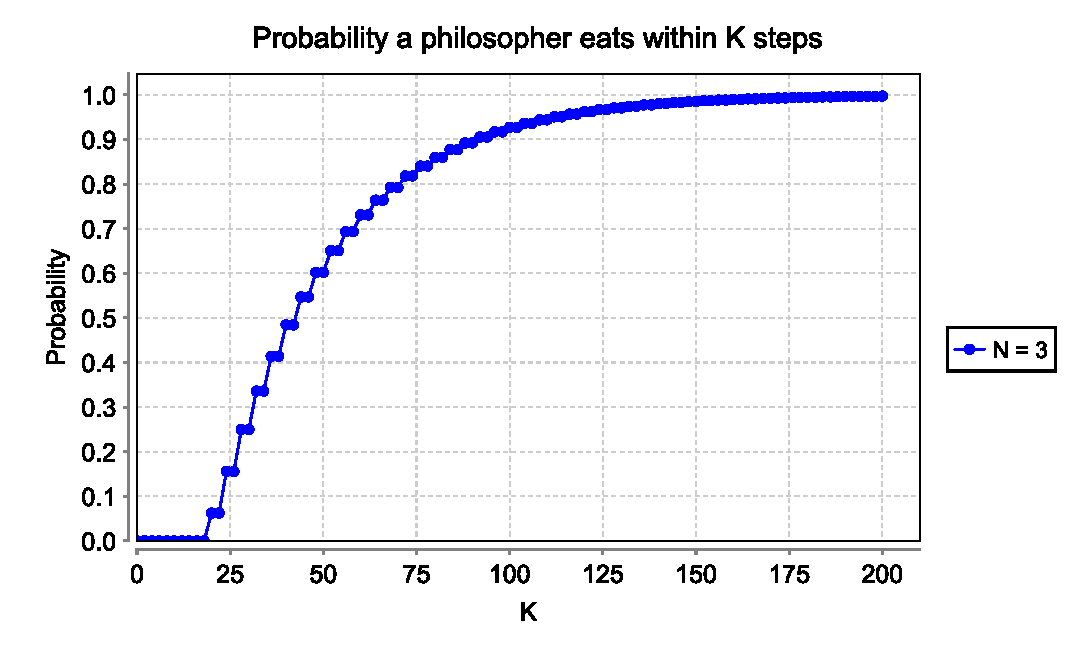
\includegraphics[width=.45 \linewidth]{case-stud-3.eps}
        & 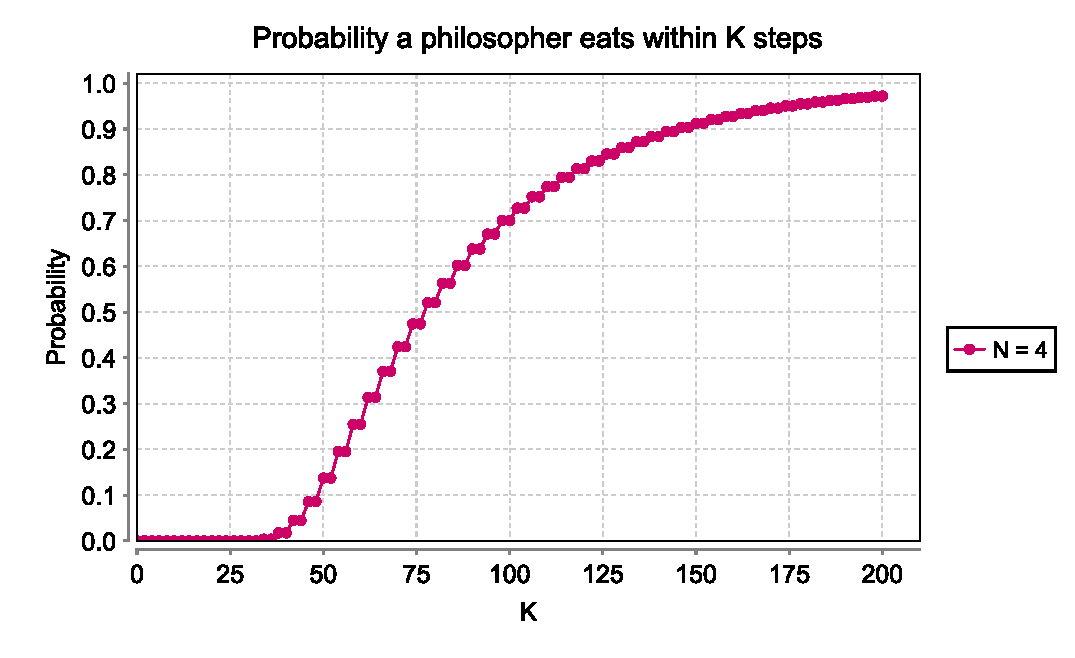
\includegraphics[width=.45 \linewidth]{case-stud-4.eps} \\
        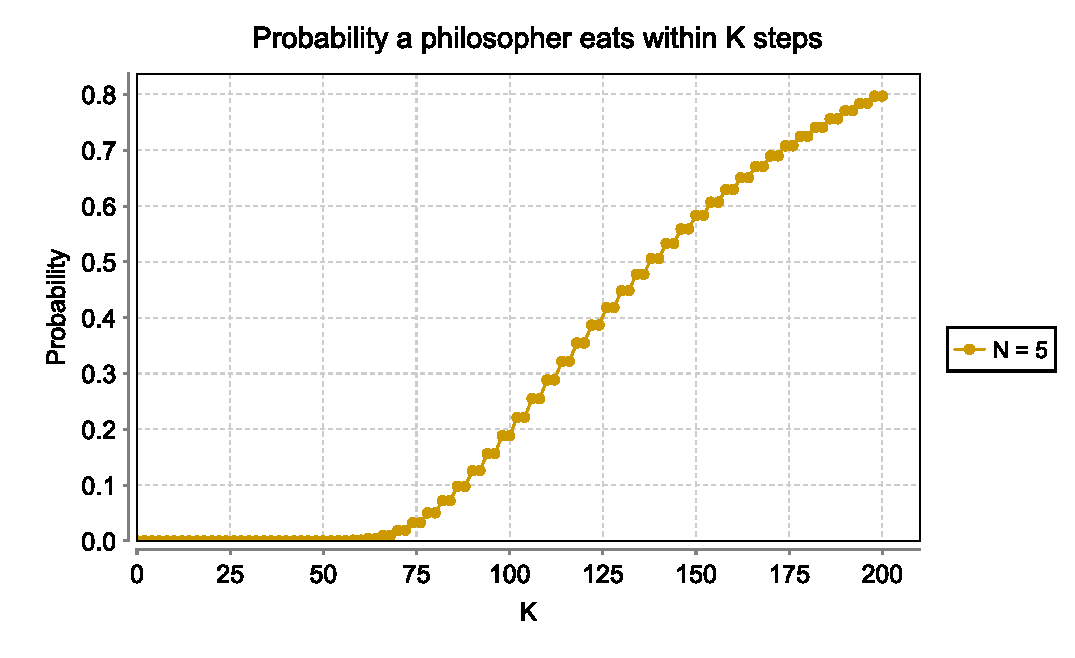
\includegraphics[width=.45 \linewidth]{case-stud-5.eps}
        & 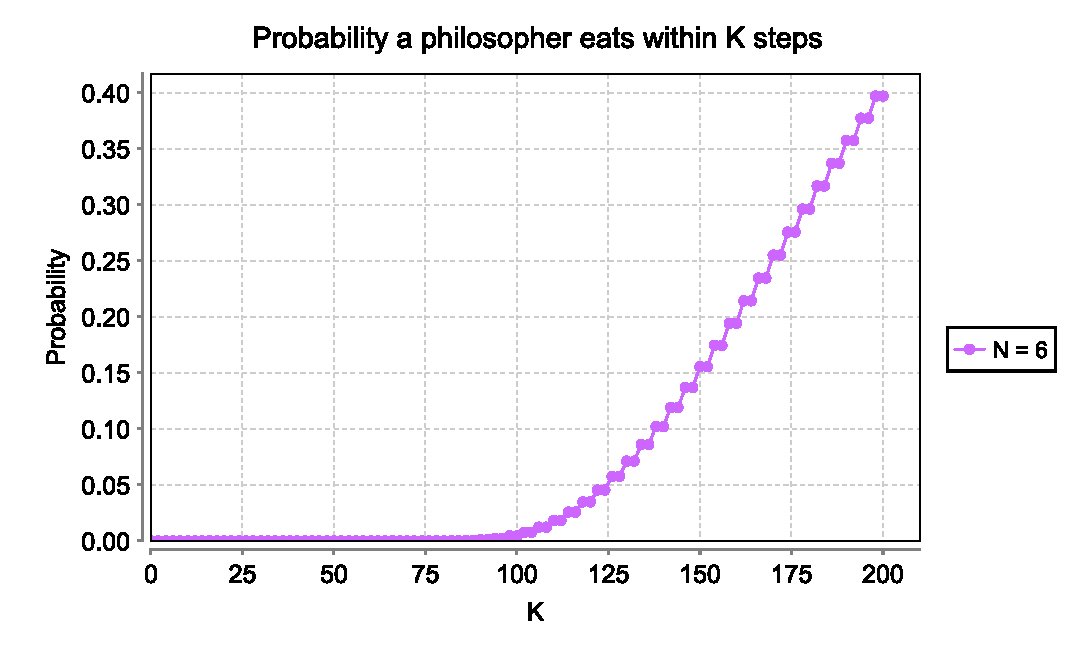
\includegraphics[width=.45 \linewidth]{case-stud-6.eps}
    \end{tabular}

    \caption{%
        Probabilities that a~philosopher eats within~$ K $ steps
        plotted for different values of~$ N $%
    }
    \label{fig:caseStudExp2}
\end{figure}

The last property decided using model checking, in this example, is
\say{From a~state where someone is hungry, what is the \emph{maximum
expected number of steps} until a~philosopher eats?} It can be
answered using the defined \emph{reward} with the following formula:
$$
    \mathrm{R}\{\texttt{"num\_steps"}\}_{\max = ?}
    [\mathrm{F}\ \texttt{"eat"}\ \{\texttt{"hungry"}\}\{\max\}]
$$
The result is $ \approx 51 $ for $ N = 3 $, $ \approx 89 $ for $ N = 4 $,
$ \approx 149 $ for $ N = 5 $, and $ \approx 244 $ for $ N = 6 $.


\section{Custom Experiments}
\label{sec:customExp}

The Chapter discusses performed custom experiments, concerned
\emph{population models}. In particular, it focuses on the modelling of
\emph{virus development}. The idea is based on the project assignment
from~\cite{mbaCeska}. A~description of the model is given in
Chapter~\ref{sec:customExpModel}. Next, experiments are described in
Chapter~\ref{sec:customExpExps}.

\subsection{Description of the Model}
\label{sec:customExpModel}

Within this project, \emph{population models} that use \emph{chemical
reaction networks} are considered, where \emph{transition rates}
correspond to \emph{mass-action kinetics}. Here is a~very simplified
example: it is given a~chemical reaction network $ A + B
\xrightarrow{k} C $, where $ A, B, C $ are some species. That means
that~$ A $ and~$ B $ together products~$ C $. And a~transition rate
is $ r = |A| \cdot |B| \cdot k $.

In the considered model, there is virus development in a~\emph{closed
population}. The population contains
\begin{enumerate*}[label={(\roman*)}]
    \item
        \emph{healthy individuals ($ Z $)} that can be infected,

    \item
        \emph{infected individuals ($ N $)} that can be healed,

    \item
        and \emph{healed individuals ($ U $)} that that can not be
        infected anymore.
\end{enumerate*}
The initial population is $ Z = 95 $, $ N = 5 $, $ U = 0 $. The
development of the virus is influenced by the following two
\emph{reactions}:
\begin{enumerate*}[label={(\roman*)}]
    \item
        \emph{infection}: $ Z + N \xrightarrow{k_i} N + N $, where
        $ k_i \in [0.001, 0.011] $;

    \item
        and \emph{healing}: $ N \xrightarrow{k_r} U $, where $ k_r \in
        [0.01, 0.11] $.
\end{enumerate*}

It is modelled as a~CTMC because these chemical reactions naturally
operate in \emph{continuous-time}. A~source code in the PRISM modelling
language is given in Listing~\ref{list:customExp}. In the code, there are
some defined constants define that the initial population, and undefined
constants with reactions rates, these are given during model checking
of particular properties. The model contains a~\texttt{virus}
\emph{module} that implements appropriate reaction network. There are
variables that correspond to~$ Z $, $ N $, and~$ U $. Further, there
are implemented commands that correspond to appropriate reactions.
Transaction rates in these commands are as follows (w.r.t. mass-action
kinetics): $ r_i = |Z| \cdot |N| \cdot k_i = z \cdot n \cdot k_i $,
and $ r_r = |N| \cdot k_r = n \cdot k_r $.

\begin{lstlisting}[
    language=prism, label={list:customExp}, float=h!bt, caption={%
        Virus development modelled in the PRISM modelling language%
    }
]
ctmc

// initial values
const int z_init=95;
const int n_init=5;
const int u_init=0;
const int total=z_init+n_init+u_init;

const double ki; // rate of infection
const double kr; // rate of healing

module virus
  z: [0..total] init z_init; // healthy individuals
  n: [0..total] init n_init; // infected individuals
  u: [0..total] init u_init; // healed individuals

  [] z>0 & n>0 & n<total -> z*n*ki : (z'=z-1) & (n'=n+1); // infection
  [] n>0 & u<total -> n*kr : (n'=n-1) & (u'=u+1); // healing
endmodule
\end{lstlisting}

\subsection{Performed Experiments}
\label{sec:customExpExps}

Table~\ref{tab:customExpModel} demonstrates statistics for the CTMC built
for the model.

\begin{table}[hbt]
    \centering

    \begin{tabular}{|r||r|r||r|r||r|r|}
        \hline

        \multicolumn{1}{|c||}{\multirow{2}{*}{$ k_i; k_r $}}
            & \multicolumn{2}{c||}{\textbf{Model}}
            & \multicolumn{2}{c||}{\textbf{MTBDD}}
            & \multicolumn{2}{c|}{\textbf{Construction}} \\ \cline{2-7}

        & \multicolumn{1}{c|}{\textbf{States}}
            & \multicolumn{1}{c||}{\textbf{Transitions}}
            & \multicolumn{1}{c|}{\textbf{Nodes}}
            & \multicolumn{1}{c||}{\textbf{Leaves}}
            & \multicolumn{1}{c|}{\textbf{Time (s)}}
            & \multicolumn{1}{c|}{\textbf{Iterations}} \\ \hline \hline

        0.011; 0.11 & 5,136 & 10,076 & 104,598 & 1,241 & 0.266
            & 196 \\ \hline
    \end{tabular}

    \caption{%
        Statistics for the CTMC model built for the virus development
        model%
    }
    \label{tab:customExpModel}
\end{table}

Firstly, it was model checked the following: \say{What is the probability
that the infection \emph{eventually disappears}?}. It was specified using
the formula:
$$
    \mathrm{P}_{= ?} [\mathrm{F}\ n = 0]
$$
The outcome is plotted to the graph in Figure~\ref{fig:customExpsExp1},
where~$ k_i $ and $ k_r $ range in proper intervals. It is evident
that the infection \emph{eventually, indeed disappears}.

\begin{figure}[hbt]
    \centering
    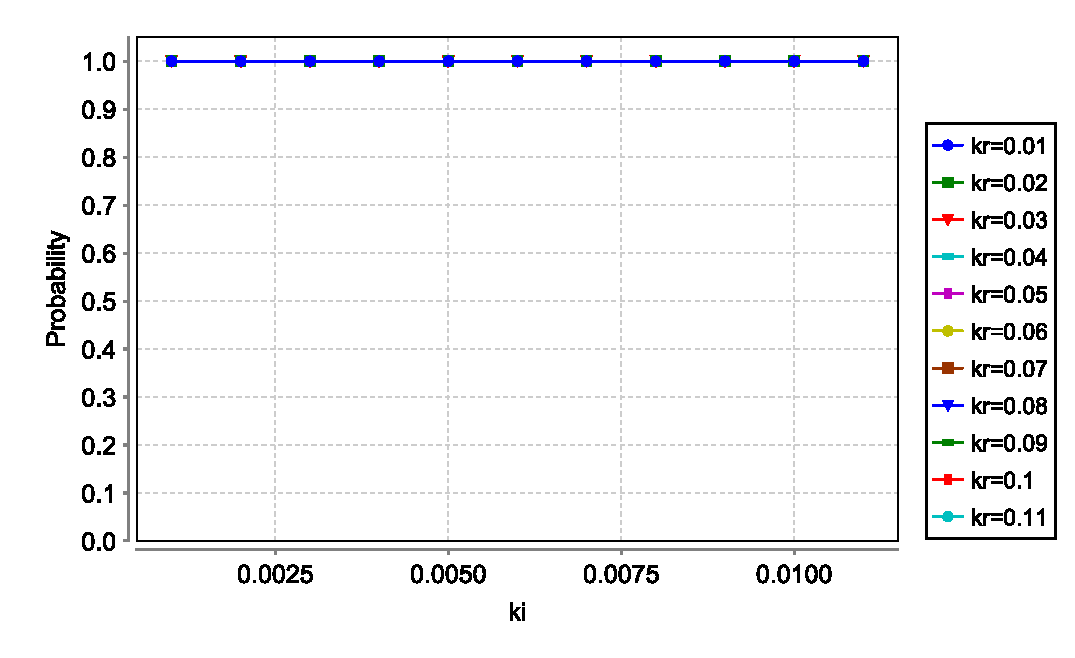
\includegraphics[width=.7 \linewidth]{custom-exp-1.eps}
    \caption{%
        The probability of the disappearance of the infection plotted
        for different values of parameters~$ k_i $ and~$ k_r $%
    }
    \label{fig:customExpsExp1}
\end{figure}

Furthermore, it was computed \say{What is the probability that the
infection \emph{takes at least}~100 time units, and it
\emph{disappears to}~120 time units?}. For this, it was constructed
the following formula:
$$
    \mathrm{P}_{= ?} [n > 0\ \mathrm{U}^{[100, 120]}\ n = 0]
$$
The result of this model checking is visible on the plotted graph
in Figure~\ref{fig:customExpsExp2}. Again, the parameters rage over
the permissible intervals.

\begin{figure}[hbt]
    \centering
    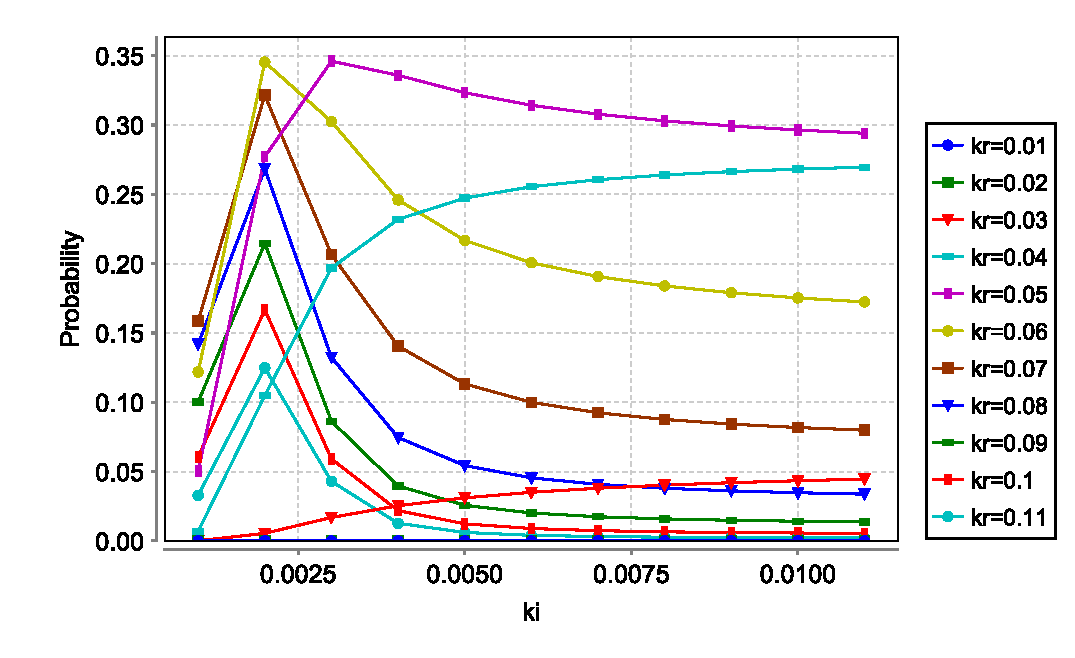
\includegraphics[width=.7 \linewidth]{custom-exp-2.eps}
    \caption{%
        The probability that the infection takes at least~100 time units,
        and it disappears to~120 time units%
    }
    \label{fig:customExpsExp2}
\end{figure}


\section{Conclusion}
\label{sec:con}

This essay sums up the \emph{probabilistic model checker} PRISM and its
usage. In the first part, it discusses \emph{probabilistic models}
and \emph{logic} that PRISM support. Moreover, it briefly describes
implementation techniques used in PRISM together with the PRISM
\emph{modelling language}. In the next parts, it describes some
performed experiments which partially outlines features of PRISM. In
particular, there is a~case study from \emph{randomised distributed
algorithms}, where the system is modelled as a~\emph{Markov decision
process}; and experiments with \emph{population models} that use
\emph{chemical reaction networks}, i.e., the system is modelled as
a~\emph{continuous-time Markov chain}.


\clearpage
\bibliographystyle{englishiso}
\bibliography{xharmi00}


\end{document}
